\documentclass[11 pt]{extarticle}

\usepackage[margin=1in]{geometry}
\usepackage{amsmath,amsthm,amssymb}
\usepackage[shortlabels, inline]{enumitem}
\usepackage{mleftright}
\usepackage{array}
\usepackage{gensymb}
\usepackage[english]{babel}
\usepackage{setspace}
\usepackage{pgfplots}
\usepackage{booktabs}
\usepackage[numbers]{natbib}
\usepackage{listings,xcolor}
\usepackage{todonotes}
\newcommand\mdoubleplus{\mathbin{+\mkern-10mu+}}
\usepackage{tikz-cd}
% http://tex.stackexchange.com/q/169557/5764
\usepackage{mathtools}
\DeclarePairedDelimiter{\norm}{\lVert}{\rVert}
\newcommand{\vectorproj}[2][]{\textit{proj}_{\vect{#1}}\vect{#2}}
\newcommand{\vect}{\mathbf}
\pgfplotsset{width=10cm,compat=1.9}


\newcommand{\N}{\mathbb{N}}
\newcommand{\Z}{\mathbb{Z}}
\newcommand{\R}{\mathbb{R}}
\newcommand{\C}{\mathbb{C}}
\newcommand{\Q}{\mathbb{Q}}
\newcommand{\Mat}{\text{Mat}}
\newcommand{\sgn}{\text{sgn}}
\DeclareMathOperator{\lcm}{lcm}
\DeclareMathOperator{\img}{im}

\let\hom\relax% Set equal to \relax so that LaTeX thinks it's not defined
\DeclareMathOperator{\hom}{Hom}
\newcommand{\Char}{\text{char}}
\newcommand{\defeq}{\overset{\text{\tiny def}}{=}}

\theoremstyle{remark}
\newtheorem{lemma}{Lemma}


\newenvironment{amatrix}[1]{%
  \left[\begin{array}{@{}*{#1}{c}|c@{}}
          }{%
        \end{array}\right]
    }

    \renewcommand\qedsymbol{$\blacksquare$}

    \newenvironment{theorem}[2][Theorem]{\begin{trivlist}
      \item[\hskip \labelsep {\bfseries #1}\hskip \labelsep {\bfseries #2.}]}{\end{trivlist}}
    \newenvironment{theorem*}[1][Theorem:]{\begin{trivlist}
      \item[\hskip \labelsep {\bfseries #1}]}{\end{trivlist}}
    \newenvironment{exercise}[2][Exercise]{\begin{trivlist}
      \item[\hskip \labelsep {\bfseries #1}\hskip \labelsep {\bfseries #2.}]}{\end{trivlist}}
    \newenvironment{reflection}[2][Reflection]{\begin{trivlist}
      \item[\hskip \labelsep {\bfseries #1}\hskip \labelsep {\bfseries #2.}]}{\end{trivlist}}
    \newenvironment{proposition}[2][Proposition]{\begin{trivlist}
      \item[\hskip \labelsep {\bfseries #1}\hskip \labelsep {\bfseries #2.}]}{\end{trivlist}}
    \newenvironment{corollary}[2][Corollary]{\begin{trivlist}
      \item[\hskip \labelsep {\bfseries #1}\hskip \labelsep {\bfseries #2.}]}{\end{trivlist}}

    \begin{document}
\onehalfspacing

\title{Zero-Knowledge Credentials for Smart Contracts}
\author{Lucas Switzer, Tjaden Hess}

\maketitle

\begin{abstract}
	Public blockchains present unique opportunities for the implementation of
	autonomous and trustless systems, but suffer from trade-offs between
	privacy and expressivity. In this paper we present an implementation of a
	zkSNARK-based
	anonymous credential scheme for the Ethereum blockchain and give
	benchmarks for usage costs. We present as an example application an
  age-verification contract.
\end{abstract}

\section{Introduction}
While blockchains have found use cases in publicly accessible distributed
systems, they pose a challenge in that due to their public nature it is
currently impossible to attest to aspects of one's identity without the
participation of a trusted credential issuer. Many distributed applications have
some responsibility to verify aspects of their users' identity, such as age or
place of residence, but would ideally not reveal anything else about the user,
including metadata about past and future attestations of identity.

\subsection{Prior Work}
Identity systems for public blockchains have been proposed before in the form of
serivces like Civic\cite{CivicSecureIdentity} and Uport\cite{braendgaardDifferentApproachesEthereum2018}, wherein users can acquire attestations from
trusted issuers about facets of their identity (name, age, country of origin,
etc). These services promise ``anonymous'' attestation, but are
\textit{linkable}, i.e.\ multiple attestations by the same user are trivially
identifiable, and \textit{pseudonymous}, i.e.\ attestations are
linked to a pseudonym that is known by the credential issuer. If a credential
issuer leaks their records, then all past activity by a user is deanonymized.

A zero-knowledge credential scheme for blockchains was proposed by
\citet{garmanDecentralizedAnonymousCredentials2013}, using zkSNARKS. Our system
adapts this scheme for the Ethereum\cite{woodEthereumSecureDecentralised2014} blockchain and implements more expressive
forms of credentials that can be easily utilized for ad-hoc attestations in zero-knowledge.

\subsection{Protocol Overview}
\subsubsection{Actors}
The major actors in this protocol are \textit{issuers}, \textit{verifiers} and
\textit{users}. A verifier is a  smart-contract that wants to ensure that
users calling a function are authorized to do so. In order to authorize users,
the contract designates an issuer, who is responsible for granting credentials
to users and keeping a Merkle tree of valid credentials. The verifier then
requires that each user provide a zero-knowledge proof that the user possesses a
credential in the merkle tree with attributes in the required range. Both
credential issuance and usage is done in zero-knowledge and attestations are
reusable and unlinkable.

\subsection{Approach}
We implement zero-knowledge proofs using the elliptic curve pairing precompiled
contracts in Ethereum, using the Pinnochio protocol
\cite{parnoPinocchioNearlyPractical2013}. We constructed the arithmetic circuits
for the proofs using libsnark \cite{ben-sassonSNARKsVerifyingProgram2013}.
Commitment trees are stored using IPFS \cite{benetIPFSContentAddressed2014}.



\section{Implementation}

\subsection{Credentials}


\subsubsection{Credential Contents}
Each credential is of the form
\begin{equation*}
c =  ( \texttt{sk}, \{attr_1, \dots, attr_n\})
\end{equation*}

where $\texttt{sk} \in \{0, 1\}^\lambda$ and $attr_i \in \Z_{2^{32}}$.

\subsubsection{Credential Requests}
A credential request is a tuple of the form
\begin{equation*}
  r = (\texttt{merkle\_root}, \{u_1, \dots,u_n\}, \{\ell_1,\dots,\ell_n\}, S, k\_bound)
\end{equation*}

where $\texttt{merkle\_root}$ is the root of a Merkle-tree of valid credential
commitments, $u_i, \ell_i \in \Z_{2^{32}}$ are bounds on acceptable attribute
values, $S$ is a request-specific salt, and $k\_bound\in \N$ is the allowed number of
uses of a single credential per salt $S$.

\subsubsection{k-show Credentials}
Every proof $\pi$ that a user generates has as public input
$\texttt{serial}_\pi$ which is defined as
\begin{equation*}
  H(\texttt{sk}_u || S_v || k)
\end{equation*}

and a public input $\texttt{k\_bound}$ such that $k\leq \texttt{k\_bound}$. For
each proof that the verifier accepts, the verifier adds $\texttt{serial}_\pi$ to
its nullifier set $N$. A verifier accepts $\pi$ only if $\pi \notin N$. Thus,
for a given salt $S_v$ the user may produce up to $\texttt{k\_bound}$ distinct
valid proofs, while remaining unlinkable. The verifier $v$ may select $S$ such
that it changes over time, for instance such that it contains the hash of the
most recent block with height a multiple of 1 million, which allows for
rate-limited credentials.

\subsubsection{Bounded-attributes}
A proof for a given credential request $r$ must assert that $attr_i \in [\ell_i,
u_i]$ for all $1\leq i\leq n$. This allows attestations such as ``I possess over
\$1 million'', ``I am between the ages of 21 and 45'', or ``I live in the USA'',
without revealing any additional information.

\subsubsection{Arithmetic Circuit}
The verification algorithm for credentials is encoded as a rank-1 constraint
system, and accepts as public input a credential request $r$ along with a serial
number \texttt{serial}, and as private
input
\begin{equation*}
  aux = (c, k, M)
\end{equation*}
where $c$ is the credential satisfying request $r$, $k$ is the nonce that
generates $\texttt{serial}$, and $M$ is a merkle proof giving the authentication
path for $c$. The circuit constrains
\begin{itemize}
\item $M$ to be a valid merkle proof for $c$ in
  the tree with root $\texttt{merkle\_root}$
\item $k \leq k\_bound$
  \item  $\ell_i\leq
    attr_i\leq u_i$
  \item \texttt{serial} = $ H(\texttt{sk}_u || S_v || k)$
\end{itemize}

The verifier accepts if the proof satisfies this circuit and \texttt{serial} is
not in its nullifier set $N$.


\subsection{The ZKID Service}
\begin{figure}[h]
  \centering
  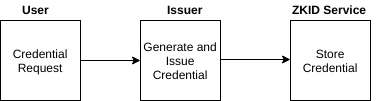
\includegraphics[scale=0.5]{issuing}\vspace{40pt}
  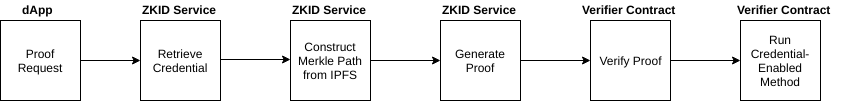
\includegraphics[scale=0.5]{verifying}
  \caption{ZKID Service}
\end{figure}
\subsubsection{JSON RPC}

The ZKID client application acts as a JSON RPC service that can handle requests from client dApps. For the simplest implementation,
the RPC service offered a single procedure: GenerateProofs. This procedure takes as input all the fields nessesary
to construct the required set of public inputs for the proofs. If proof generation was successful, the service will respond with a 
set of generated proofs and relevant public inputs. The returned proofs can then be sent to the verifier contract.  

\subsection{Verifiers}

It is expected, although not required, that credential-enabled contracts perform their own proof verification. For this reason, we have
developed a Solidity library that enables contracts to verify proofs autonomously. The verifier library follows a scheme similar to that
of Zokrates [insert citation here]. The library exposes a single method to be utlized by the higher-level contract: verifyTx. This 
method does precisely what the name implies and verifies as set of proofs encoded as bytes and returns true if all proofs where sucessfully
verified and false otherwise. 

It is important to note that all verification calculations are done on-chain and therefore can potentially require immense amounts of gas.
For this reason, the number of proofs requested for verification should be kept to a minimum. 

\subsection{Issuers}

Although there is no strict template for an issuer (asside from the credential contruction), we purpose a scheme that we believe
will offers most of the elementary functions of an issuer. This basic scheme involves 2 main functions:
credential-holder stake and distributed merkle tree storage.

\subsubsection{Credential-Holder Stake}

An obvious vulenerability of the credential system as described is the ability to share credentials. So, for example, an uncredible could may
a credible party for a specific credential. We proprose that an issuer's require a credential-requester to submit a stake when 
applying for a credential. This stake can be redeemed by an user that can provide the issuer contract with a specified pre-image. Once 
redeemed, the credential because invalidated. Therefore, if a dishonest party were to give away their credential, the new holder of the credential
could steal the original holder's stake. This requires issuers to set their stakes high enough such that no party would be willing to pay the
price of the stake for the credential. A stake system could also lead to varying "tiers" of issuers where issuers that require higher stakes could be 
percieved as having higher credibility do the lower probability of users sharing said issuer's credential.

\subsubsection{InterPlanetary File System (IPFS)}

As designed, the ZKID service expects verifiers to store their issued-credential merkle trees using the distributed file system service, InterPlanetary File System (IPFS).
By utilizing IPFS, the ZKID service promotes the distributed nature of its environment and further encourages issuers to take advantage of said distributed nature. All issuer
contracts must supply a GetMerkleTreeAddress method that returns the IPFS address of their merkle root. Every issuer must also append the hashes of every issued credential 
to their merkle tree so that verifiers and clients can construct merkle tree paths and subsequently merkle tree membership proofs as nessesary. 

\subsubsection{Credential Annotated ABI}
The properly interface with the ZKID Service a dApp would provide an annotated ABI for its dependant contract(s).
The annotations describe the required credentials for a given method within the smart contract and will
be used to communicate public inputs to the ZKID prooving service. An annotated ABI function
would appear as follow:

Note that the description field is not nessesary for generation / verification of proofs, but is supplied soley for
the use of the credential-acknowledgement framework described later. 

\subsubsection{ZKID web3 Framework}

To a dApp's migration to credentail-enabled contracts as smooth as possible we have supplied a ZKID framework that interfaces
with our prove-generation service and seemlessly collects and supplies verifcation arguments to credential-enabled methods. This 
allows dApp creators to integrate credential functionality without changing their already developed application code.

To utlize the framework a dApp simply replaces all existing contract calls with calls to their credential accepting counterparts. 
This can be accomplished very concisely by wrapping the credial-accepting method call with partially applied
function.

The "Join" function in the provided example application is an example of how to properly provide the ZKID framework with a partially applied credential-enabled function. Originally, took a number of non-proof arguments. 
The credential enabled join now takes the non-proof arguments as well as proof arguments. This partial application hides the non-proof arguments from the ZKID CredentialBlock and allows the CredentialBlock to 
supply the proof arguments post proof-generation. The dApp's code has now migrated its call to "Join" to a credential-enabled call with minimal additions.

\section{Benchmarks}

Deployment of our contract takes $3.6$ million gas, and a single execution of
the verifier requires $1.79$ million. At current prices this is about $0.01432$
ETH or $\$10.50$. Proving time for a tree dept of $32$ is 43.2 seconds. We feel
that these are reasonable enough for use, but could certainly be improved as
discussed below. Proving time scales linearly with the depth of the merkle tree,
while verification cost is constant.

\section{Example Application}

To demonstrate the facilities provided by the our system we developed a simple lottery dApp that requries participants to be
both over the age of 18 and have American Citizenship to participate. Along with the dApp, we created a credential-acknowledgement
framework that would allow applications to prompt users for the required credentials before any proofs are generated.



\section{Future Work}
Currently the contract does not make use of the preprocessed verifier that
libsnark provides, which would allow us to remove 2 pairing checks at the cost
of several EC group operations. Additionally, Zcash is developing a new zkSNARK
system on a more efficient curve called JubJub\cite{ZcashJubjub} that allows fixed-base
exponentiation for efficient EC operations in
circuits, allowing efficient CRHs.

\section{Acknowledgements}
Huge thanks to Ian Miers for helping set us on the right path and formalizing
the properties that an anonymous credential scheme should have.

\bibliographystyle{plainnat}
\bibliography{Identity}
\end{document}